\section{Présentation}


\subsection{Contexte d'enseignement}

Lauréat du concours du CAPES de Numérique et Sciences Informatique (NSI), je suis  cette année professeur stagiaire. Préalablement fonctionnaire de l'éducation nationale en tant que professeur en lycée professionnel (PLP) de mathématiques, sciences-physiques et chimiques, c'est dans le cadre de la formation continue des enseignants stagiaires à \emph{temps complet} que je vous propose cet écrit réflexif.

Cette année est pour moi très particulière et particulière puisque j'assiste en parallèle à certains cours du M2 MEEF avec des professeurs stagiaires à \emph{temps partiel} de NSI et sciences de l'ingénieur (SI). Bénéficiant d'une validation des acquis pour certaines unités d'enseignement (UE) ainsi que d'une dispense de cours, je travaille néanmoins sur la validation de l'UE 2, accompagné pour cela par Jean-François Herold.

J'enseigne à 18 heures dans le lycée Simone Veil de Marseille (13~013). Cet établissement de 850 élèves accueille les élèves de la seconde au BTS et admet une section professionnel.

Mon service est partagé entre :

\begin{description}
    \item[8 heures] d'enseignement de sciences numériques et technologie (SNT) auprès de quatre classes de seconde et
    \item[10 heures] d'enseignement de NSI auprès d'élèves de première et de terminale.
\end{description}

L'enseignement de NSI est un \emph{enseignement de spécialité} qui a vu le jour avec la \emph{réforme du baccalauréat général et technologique et du lycée} de 2018. Après une succession d'évolutions, de modification et d'ajustements de cette réforme, un élève de fin de seconde doit actuellement choisir trois enseignements de spécialités parmi l'ensemble des enseignements disponibles sur son secteur d'affectation. Libre a lui (et à sa famille) de reproduire les schémas traditionnels tels que :

\begin{itemize}
    \item pôle scientifique type S avec les spécialités mathématiques, physiques et sciences et vie de la terre (SVT)
    \item pôle littéraire type L avec humanité, littérature et philosophie (HLP), langue, littératures et cultures étrangères (LLCE)
    \item pole économique et social type ES avec histoire géographie, géopolitique et sciences politiques (HGGSP), sciences économiques et sociales (SES).
\end{itemize}

Néanmoins d'autres voies sont possibles et désormais l'éducation physique et sportive (EPS), les sciences de l'ingénieur (SI), la musique, l'audiovisuel ou les sciences informatiques font leur apparition auprès des spécialités typées plus traditionnelles.


\subsection{Trois constats}


\paragraph{Des élèves qui ne se connaissent pas} 
En tant qu'enseignants de spécialité, je constate que je me retrouve face à un groupe d'élèves dont les seuls moments partagés se font dans notre cours. 
\\
En effet, cette individualisation du choix couplée à la richesse de l'offre engendre une très grande variété de couplages sur les cohortes d'élèves de première et de terminale. Par exemple sur mon établissement qui propose 9 enseignements de spécialités, pas moins de 84 combinaisons différentes sont possibles. Sur ces deux niveaux, il n'existe donc plus de classe aux spécialités homogènes. C'est-à-dire qu'il n'existe plus de classes dont tous les élèves suivent les mêmes enseignements de spécialité. Les classes de spécialité sont donc devenues des \emph{groupes} de spécialités, et la très grande majorité de ces groupes sont constitués d'élèves provenant de classes différentes.
\\
Ce morcellement des classes implique que les élèves se retrouvant dans chaque groupe de spécialité se connaissent beaucoup moins. Ils ne se côtoient ensemble que pendant les heures consacrées à chaque enseignement de spécialité. Le parcours de chaque élève est donc fortement individualisé et les groupes de spécialité sont structurellement d'une constitution autre que celle de la classe entière ou de ses demi-groupes. Il me semble que le fonctionnement structurel induit par la \emph{réforme du baccalauréat général et technologique et du lycée} engendre une école cloisonnant l'individu plutôt qu'une école comme levier de promotion du collectif. 

\paragraph{Importance du socio-constructivisme} De ce premier constat émerge pour moi la réflexion suivante : cette individualisation m'apparaît clairement contradictoire avec le socio-constructivisme si important pour l'apprentissage. Un savoir se construit d'autant mieux s'il émerge d'interactions sociales. Mais si ces dernières entre les élèves sont minimales, il n'y a alors ni échange, ni partage ou encore absence d'intérêt les uns pour les autres. C'est pourquoi il m'est apparu pendant l'année primordial de favoriser les interactions entre les élèves.


\paragraph{Nécessité d'une pédagogie différenciée} Un dernier constat concernant la pratique de l'enseignement actuelle. Les institutions, tout comme la recherche, promeuvent la pédagogie différenciée. Cette différenciation est relativement aisée à penser en enseignement d'informatiques. Les environnements de travail, qu'ils soient matériels ou numériques, aident à la rendre opérationnelle.
\\
En revanche, cette différenciation semble elle aussi contradictoire avec le socio-constructivisme. Comment différencier les savoirs à enseigner et s'adapter à l'élève dans son intégralité tout en conservant une dimension socio-constructiviste ?

C'est donc fasse à ces mise en tension du socio-constructivisme, à la fois par la différenciation pédagogique et par l'individualisation structurelle des groupes de spécialité, que je me suis (entres autres) interrogé cette année. J'ai donc trouvé nécessaire de mettre en œuvre un dispositif de pédagogie différenciée qui puisse promouvoir le collectif.


\section{Méthode Jigsaw}

Parmi les différentes méthodologie proposée de pédagogie différenciée, je me suis tourné vers une pédagogie de \emph{tutorat bidirectionnel}. 

L'idée de tutorat est de créer des groupes d'élèves intégrant deux rôles symétriques : l'élève \emph{tuteur}, qui transmet un savoir, et l'élève \emph{apprenant}, qui découvre le savoir transmis par son camarade.

Pour éviter l'écueil de la stigmatisation d'un élève étiqueté \emph{bon} ou \emph{mauvais} face à ses camarades, il m'est apparu indispensable de permettre à tous les élèves de tenir chacun des deux rôles. C'est cet aspect là du tutorat que l'on qualifie de \emph{bidirectionnel}.

J'ai donc imaginé un dispositif qui s'avère ressembler énormément à la méthode \emph{jigsaw} apparue aux États-Unis.

L'idée est de découper une séance en deux moments aux objectifs bien différents :

\begin{description}
    \item[moment de l'appropriation] Dans un premier temps, des groupes d'élèves sont constitués et chaque groupe a pour objectifs de s'approprier un savoir. Chaque groupe possède un savoir différent à étudier. Durant ce moment, tous les élèves prennent connaissance au sein de leur groupe d'un savoir dont ils seront les tuteurs.
    \item[moment de la transmission] Dans un deuxième temps, on répartit tous les élèves dans d'autres groupes de façon à séparer les tuteurs. Les nouveaux groupes créés doivent posséder au moins un tuteur de chacun des savoirs concerné. Durant ce moment, chaque élève doit s'approprier l'ensemble des savoirs ce qui oblige chaque tuteur à exposer, expliquer et faire comprendre le savoir dont il est le garant.
\end{description}

Comme on peut le constater, chaque élèves est à la fois tuteur d'un savoir et apprenant de l'ensemble des autres savoirs.

Cette méthodologie permet :

\begin{itemize}
    \item une absence totale de stigmatisation entres élèves et 
    \item un échange très fort entres élèves centré sur le savoir.
\end{itemize}


Lors de la mise en œuvre d'un tel dispositif, puisque le moment d'appropriation nécessite une grande autonomie des élèves, il est indispensable de créer ces premiers groupes de façon différenciées. En effet, il faut que les élèves d'un même groupe aient des zones proximales de développement (ZPD) sécante entres elles. Pour cela, il est nécessaire de différencier les élèves.

C'est pourquoi, une première étape d'évaluation des élèves est indispensable. Lors de ce moment de la différenciation, je me suis efforcé de créer des groupes de niveaux en lien avec les prérequis nécessaires lors des moments suivants.

La méthodologie réalisée a donc été organisée en trois étapes :

\begin{description}
    \item[étape (a)] moment de la différenciation pour créer des groupes de niveaux,
    \item[étape (b)] moment de l'appropriation pour former les futurs tuteurs, par groupe de niveau, sur les savoirs à transmettre,
    \item[étape (c)] moment de la transmission pour que chaque élève transmette au sein de son groupe son savoir.
\end{description}


\begin{center}
    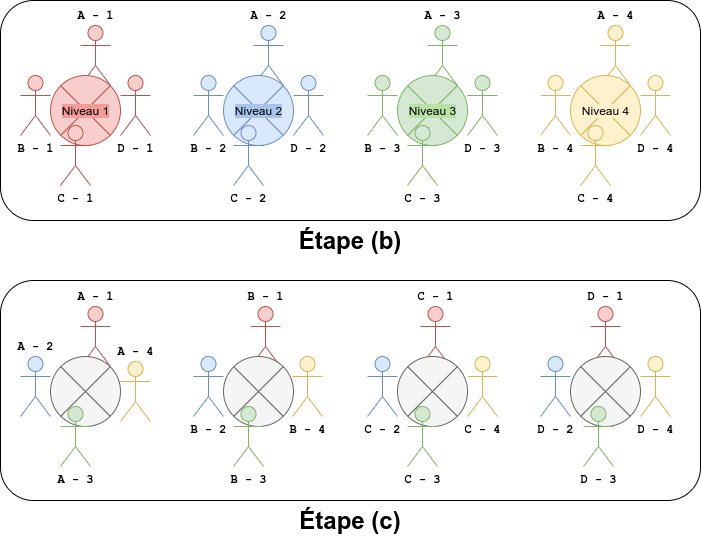
\includegraphics[width=0.5\linewidth]{res/diagramme.drawio.png}
\end{center}




\section{Première expérimentation}

\subsection{3 moments de la séances}

\subsection{Difficultés}

\subsection{Ressenti}

\section{Conclusion}